%%% use twocolumn and 10pt options with the asme2ej format
\documentclass[twocolumn,10pt]{asme2ej}

\usepackage{graphicx} %% for loading jpg figures
\usepackage{comment}
\usepackage{amsmath}
%\usepackage{algpseudocode}
\usepackage[ruled]{algorithm2e}
\usepackage{pgfplots}
\usepackage{url}
%\usepackage{hyperref}
%\graphicspath{ {../figure/} }

%% The class has several options
%  onecolumn/twocolumn - format for one or two columns per page
%  10pt/11pt/12pt - use 10, 11, or 12 point font
%  oneside/twoside - format for oneside/twosided printing
%  final/draft - format for final/draft copy
%  cleanfoot - take out copyright info in footer leave page number
%  cleanhead - take out the conference banner on the title page
%  titlepage/notitlepage - put in titlepage or leave out titlepage
%  
%% The default is oneside, onecolumn, 10pt, final


\title{Genetic Algorithms for a Discrete Lot Sizing Problem}

%%% first author
\author{Norbert HOUNKONNOU
    \affiliation{
	University of Abomey-Calavi\\
    }	
}

%%% second author
%%% remove the following entry for single author papers
%%% add more entries for additional authors
\author{Vinasetan Ratheil HOUNDJI
\thanks{Address all correspondence related to ASME style format and figures to this author.} 
    \affiliation{
    University of Abomey-Calavi
    }
}

%%% third author
%%% remove the following entry for single author papers
%%% add more entries for additional authors
\author{Tafsir GNA\\
        Research Assistant\\
}


\begin{document}

\maketitle    

%%%%%%%%%%%%%%%%%%%%%%%%%%%%%%%%%%%%%%%%%%%%%%%%%%%%%%%%%%%%%%%%%%%%%%
\begin{abstract}
{\it Lot sizing takes an important place in production planning in industry. It consists
in determining a production plan that meets the orders and at the same time takes
into account the financial objectives of the enterprise. Recent researches have experimented an NP-Hard variant of lot sizing problem: the Pigment Sequencing Problem
(PSP). Several methods have been applied to PSP. None of the applied methods is
based on genetic algorithms whereas they showed their efficiency in solving optimization problems. In this document, we apply a solving method based on genetic algorithms to PSP.
The experiments allow us to compare the results obtained in applying this
solving method to the ones obtained of the application of another method implemented in
earlier researches: The Constraint Programming (CP). These very first results show that genetic algorithms are promising in solving PSP. \\
\textbf{Key-words}: Genetic algorithm, production planning, pigment sequencing problem, lot
sizing.
}
\end{abstract}

%%%%%%%%%%%%%%%%%%%%%%%%%%%%%%%%%%%%%%%%%%%%%%%%%%%%%%%%%%%%%%%%%%%%%%

\begin{comment}
    \begin{nomenclature}
    \entry{A}{You may include nomenclature here.}
    \entry{$\alpha$}{There are two arguments for each entry of the nomemclature environment, the symbol and the definition.}
    \end{nomenclature}
    
    The primary text heading is  boldface and flushed left with the left margin.  The spacing between the  text and the heading is two line spaces.
\end{comment}

%%%%%%%%%%%%%%%%%%%%%%%%%%%%%%%%%%%%%%%%%%%%%%%%%%%%%%%%%%%%%%%%%%%%%%
\section{Introduction}

Lot sizing problem consists in identifying items to produce, when to produce and on which machine in order to meet the orders while taking into account financial goals. Such a problem has been studied these recent decades. In fact, solving a lot sizing problem has a lot of challenges. Not only several types of items are required to be produced but the production planning has to meet often opposite goals such as serving customer needs and minimizing production and stocking costs.\\
Several versions of lot sizing problems have been proposed in the literature. Lately,  Houndji et al. \cite{ratheil_stocking_paper}
et Ceschia et al. \cite{ceschia_opthub} have worked a NP-Hard variant known as \emph{Pigment Sequencing Problem}  (Pochet
et Wolsey \cite{wolsey_mip_paper}) and included in the CSPlib library (Gent and Walsh, \cite{gent_walsh_paper}). It consists in producing several items on a single machine whose production capacity is restricted to one item per period. The planning horizon is discrete and finite with stocking costs and setup costs from one item to another. \\
Pigment Sequencing problem, like any lot sizing problem can be formalized and solved with genetic algorithms. Genetic algorithms are heuristic search methods inspired by the natural evolution of living species. Based upon the concept of the survival of the fittest, genetic algorithms are able over multiple generations to find the best solution to a problem. Several researches \cite{mendes_paper} \cite{non_binary_paper} have showed how effecient they can be in solving optimization problems. \\
In this paper, we expose a search method based on genetic algorithms, then use and experiment this approach and the results obtained show that genetic algorithms are a promising method in solving a discrete lot sizing problem such as Pigment Sequencing Problem.  \\
This paper is organized as follows: Section 2 exposes some background on the Pigment Sequencing Problem, Section 3 gives details on our method based on genetic algorithms, Section 4 presents some experimental results obtained from the application of our method and Section 5 concludes and provides some perspectives.


%%%%%%%%%%%%%%%%%%%%%%%%%%%%%%%%%%%%%%%%%%%%%%%%%%%%%%%%%%%%%%%%%%%%%%
\section{Pigment Sequencing problem (PSP)}

In this section, we present the Pigment Sequencing Problem and give a formal description of the problem.

%%%%%%%%%%%%%%%%%%%%%%%%%%%%%%%%%%%%%%%%%%%%%%%%%%%%%%%%%%%%%%%%%%%%%%
\subsection{Literature review}

PSP belongs to the category of Discrete Lot Sizing Problems (DLSP). PSP is a problem in which all capacity available for a period is used to produce one item.\\
Miller and Wolsey \cite{miller_paper} formulated the DLSP with setup costs not dependent of sequence as a network flow problem. They exposed MIP formulations for various modifications (with backlogging, with safety stock, with initial stock). In addition, several more MIP formulations and variants have been proposed and discussed by Pochet and Wolsey \cite{wolsey_mip_paper}. \\
Gicquel and al. \cite{gicquel_paper} exposed a formulation and derived valid inequations for the DLSP with several items and sequential setup costs and periods, which is a modification of the problem proposed by Wolsey \cite{wolsey2_paper}. Furthermore, Gicquel and al. \cite{gicquel2_paper} proposed a new approach to the modelisation of the DLSP with several items and sequential setup costs and periods that take into account relevant physical attribute such as color, dimension and level of quality. This allowed them to effectively reduced the number of variables and constraints in the MIP Models.
Houndji and al. \cite{ratheil_stocking_paper} introduced a new global constraint they named \emph{stocking cost}  in order to effectively solve the PSP with constraint programming. They tested it on new instances and published it on CSPlib (Gent and Walsh \cite{gent_walsh_paper}). The experimental results showed that \emph{stocking cost} is effective in filtering compared to other constraints largely used in the community of constraint programming. \\
Lately, Ceschia and al. \cite{ceschia_sa_paper} applied the simulated annealing to the PSP. They introduced an approach that guides the local search and applied it to new instances available on  Opthub library \cite{ceschia_opthub}.  

%%%%%%%%%%%%%%%%%%%%%%%%%%%%%%%%%%%%%%%%%%%%%%%%%%%%%%%%%%%%%%%%%%%%%%
\subsection{Description}

Several studies \cite{houndji_paper} \cite{ceschia_sa_paper} have already been conducted on PSP. It can be described as a problem which consists in finding a production planning of various items on one machine with setup costs. Setup costs are costs necessary for the transition from an item \emph{i} to another item \emph{j} so that $ \emph{i} \neq \emph{j} $. The production planning needs to meet the customer orders while:
\begin{itemize}
  \item - not exceeding the production capacity of the machine.
  \item - minimizing the setup and stocking costs.
\end{itemize}
It is assumed that the production period is short enough to produce only one item per period and all orders are normalized i.e. the machine's production capacity is restricted to one item per period and $ d(i, t) \in \{0, 1\} $ with \emph{i} the item and \emph{t} the period. It is a production planning problem with the following specifications: a discrete and finite planning horizon, some capacity constraints, a deterministic and static order, several items and small bucket, setup costs, only one level, without shortage.\\

\textbf{Example}: Consider the following tiny problem:
\begin{itemize}
    \item - Number of items: $ NI = 2 $;
    \item - Number of periods: $ NT = 5 $;
    \item - Order per period. Be d(\emph{i}, \emph{t}) the order of item \emph{i} in the period \emph{t}: $ d(1, t ) = (0, 1, 0, 0, 1) $ and $ d(2, t) = (1, 0, 0, 0, 1)$; 
    \item - Stocking cost. Be \emph{h(i)} the stocking cost of the item i, $ h(1) = h(2) = 2 $
\end{itemize}

    Be \emph{xT} the production planning which represents a potential solution to the problem. It is a table of size \emph{NT}. A possible solution to the problem is $ xT = (2, 1, 2, 0, 1) $ with a cost of $ q(2, 1) + q(1, 2) + q(2, 1) + 2 \* h(2) = 15 $. The optimal solution is : $ xT = (2, 1, 0, 1, 2) $ with a cost of $ q(2, 1) + q(1, 2) + h(1) = 10 $.


\section{Genetic Algorithms}
Genetic algorithms are stochastic search algorithms designed to mimic the natural evolution of living species and reproduction mecanisms. They have been proposed for the first time by John Holland \cite{john_h_paper} in 1970. One of the main principles of these algorithms is the concept of the "\emph{survival of the fittest}" which states that one individual whose features fit the best with the environment is more likely to survive. Emulating the process of natural evolution, Genetic Algorithms induce the random exchange of genetic material among individuals of the same population.
This section exposes its implementation in the context of optimization problems with concepts such as \emph{Initialization}, \emph{Selection}, \emph{Crossover} or \emph{Mutation}.
 
\subsection{Initialization}
The initialization process consists of creating the first population which is a set of individuals (potential solutions). There are several strategies when creating the initial population. The initialization can be mainly random or heuristic [?]. Random initialization means that solutions which are usually a sequence of numbers, are "seeded" without any logic driving the process whilst respecting all constraints set by the problem. 
Heuristic initialisation, on the opposite is a deterministic method of initializing the population using heuristics to determine the best potential solutions close enough to optimal solutions. \\
The design of the initialization process plays a significant role in the the overall success of the implementation of genetic algorithms.

\subsection{Selection}
Selection consists of choosing the individuals from a given population for later breeding. Individuals are picked based on their fitness. Individuals with better genetic material are more likely to be chosen. There are various selection methods among which the "\emph{Roulette wheel}" method is the most common. It consists of assigning a probability to each individual of the population based on the fitness.

\subsection{Crossover}
Crossover occurs after two or more individuals have been selected for breeding. The process produces offsprings through the combination of the genetic material of the selected individuals. Several strategies can be used to generate the offsprings. The crossover process can be single-point, two-points or k-point or be uniform. 

\subsection{Mutation}

Mutation is a genetic operator that randomly alter the genetic material of randomly selected individuals. Doing so, Mutation strives to infuse diversity into the population over generations. Ultimately, Mutation is designed to avoid premature convergence in the population and the trap of a local optima.

\subsection{Termination}
Several conditions can be used to stop or terminate genetic algorithms. It can, for example, be decided to stop a genetic algorithm once a convergence occured, meaning that all the individuals in the population are similar or after a fixed number of generations. The figure \ref{fig:gaRepr} summarizes all these concepts. 

\begin{figure}[h]
    \centering
    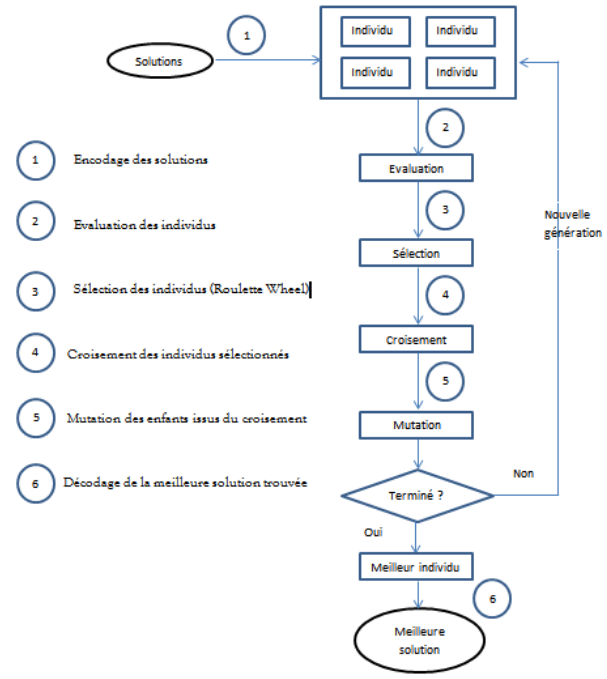
\includegraphics[scale=.3]{figure/ga_repr.png}
    \caption{Flow chart of genetic algorithms}
    \label{fig:gaRepr}
\end{figure}


%%%%%%%%%%%%%%%%%%%%%%%%%%%%%%%%%%%%%%%%%%%%%%%%%%%%%%%%%%%%%%%%%%%%%%
\section{Our Method}
In this section, we describe the mathematical model of PSP that we followed when designing our approach based on genetic algorithms. Then, we present each aspects of our application of genetic algorithms to solve PSP.

\subsection{The Mathematical Model}

Our approach based on genetic algorithms follows the first formulation of Mixed Integer Problems MIP1 model as exposed by Pochet and Wolsey [?] which states the following: 
\begin{gather}
    min (\sum_{i,j,t} q^{i,j} {X_t}^{i,j} + \sum_{i,t} h^{i} {s_t}^{i}) \\
    {s_0}^{i} = 0, \forall i \\
    {x_t}^{i} + {s_{t-1}^{i}} = {d_t}^i + {s_t}^i, \forall  i,t \\
    {x_t}^i \leq {y_t}^i, \forall  i,t \\
    \sum_{i} {y_t}^i = 1, \forall t \\
    {X_t}^{i,j} = {y_{t-1}^i} + {y_t}^j - 1, \forall i, i, t \\
    x,y,X \in {0,1}, s \in N, i \in {0,...,NI}, t \in {1,...,NT}
\end{gather}

along with the following variables:
\begin{itemize}
    \item - ${x_t}^i$: binary production variable that is 1 if the item \emph{i} is produced in the period \emph{t} and 0 otherwise;
    \item - ${y_t}^i$: binary setup variable that is 1 if the machine is set for the production of the item \emph{i} and 0 otherwise;
    \item - ${s_t}^i$: integer variable that represents the number of item \emph{i}  stored in the period \emph{t};
    \item - $q^{i,j}$: the changeover cost from item \emph{i} to item \emph{j} with $i,j \in \{0,...,NI\}$;
    \item - ${d_t}^i$: binary variable that is 1 if the item \emph{i} is ordered in the period \emph{t} and 0 otherwise;
    \item - $h_i$: the holding cost of the item \emph{i} with $i \in \{1,...,NI\}$;
    \item - ${X_t}^{i,j}$: binary variable that is 1 if in the period \emph{t}, we transitioned from the production of item \emph{i} to the one of item \emph{j} and 0 otherwise
\end{itemize}
The goal is to minimize the overall holding costs and setup costs which is expressed by the first constraint (1). The constraint (2) clearly states that there is no initial stock. The constraint (3) expresses the rule of flow conservation. The constraint (4) aims to get the setup variable ${y_t}^i$ to equal 1 if the item \emph{i} is produced in the period \emph{t}. The constraint (5) makes sure the machine is always set for an item to be produced. Therefore, ${y_t}^i$ is bound to take the value that minimizes the changeover cost. Furthermore, if there is no production in the period \emph{t}, ${y_t}^i = {y_{t-1}}^i$ or ${y_t}^i = {y_{t+1}}^i$. Thus, it is interesting to setup the machine for production even if there is no item to produced. The constraint (6) sets values to changeover variables. If ${y_{t-1}}^i$ and ${y_t}^i$ equal 1, then ${X_t}^{i,j}$ is bound to equal 1 otherwise ${X_t}^{i,j}$ would equal 0 thanks to the goal function that minimizes the changeover cost.

\subsection{Implementation}

\subsubsection{Genetic representation}

When applying genetic algorithms to a problem, finding the right representation for the individual is important and influence the efficiency of the whole algorithm. One of the simplest representation used in genetic algorithms is the one used by John Holland \cite{jh_paper} : the bit-array representation where a chromosome is represented by a string of bit containing 0 and 1 to express if an item $i$ has been produced at a given period $t$ as pictured by the following image \ref{fig:chromRepr}.

\begin{figure}[h]
    \centering
    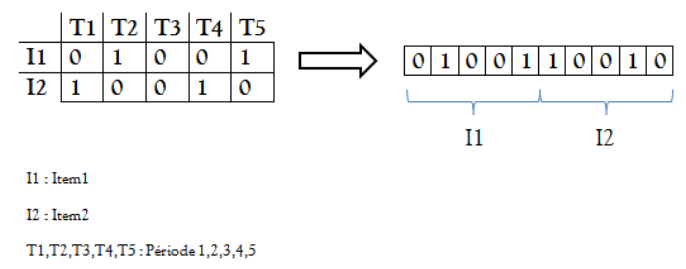
\includegraphics[scale=.3]{figure/chrom_repr.png}
    \caption{chromosome bit-array representation}
    \label{fig:chromRepr}
\end{figure}

Although nice, this representation significantly increases the complexity of the whole algorithm forcing use to go through a list of $nT * nI$ items with \emph{nT: the number of periods} and \emph{nI: the number of items}. All of this prompted the emergence of another representation as used by Mirshekarian and al \cite{non_binary_paper} in which the chromosome is represented by a string of integers of the length of the planning horizon (\emph{nT}). In this string, each integer corresponds to a indice of the item that has been produced at the exact period. Thus, the complexity is considerably reduced.  

\subsubsection{Initialization}

As stated earlier, the initialisation process consists of generating the initial population. To do so, we have opted for the heuristic algorithm based on the bread-first search technique as described here in the algorithm \ref{algo:initialisation}. The process starts at the end of the planning horizon and backtracks to the first period of production. The goal is to seed the best possible individuals for the initial population. At every step of the process, the algorithm determines which of the next children nodes are the best to expand on. Compared to a random seeding, this process produces better individuals, helping bootstrap the overall search process.

\begin{algorithm}[!ht]
\DontPrintSemicolon
    %\KwInput{Your input}
    \KwData{Expected population size, PSP instance}
    \KwResult{Population}
    %$\sum_{i=1}^{\infty} := 0$ \tcp*{this is a comment}
    %\tcc{Now this is an if...else conditional loop
    %\tcc{Now this is a While loop}
    $population \gets []$ \;
    $queue \gets firstNode(PSP\_Instance) $ \;
    $popCounter \gets queue.length $ \;
    \While{$population.length < Expected\_Population\_Size$}
    {
        \If{queue.empty}{
            break \;
        }
        $node \gets queue.popFirst()$ \\
        $popCounter \gets popCounter - 1 $ \\
        \If{node is leafNode}{
            population.add(node.chromosome) \;
            continue
        }
        \For{child in node.children(PSP\_Instance)}{
            queue.append(child) \;
            $popCounter \gets popCounter + 1 $ \\
            \If{$popCounter > Expected\_Population\_Size $}{
                break \;
            }
        }
        
       	% Do something\;
    }

\caption{Initial population algorithm}
\label{algo:initialisation}
\end{algorithm}

\subsubsection{Selection}

The selection operator we chose to implement is based the process commonly known as the "Roulette wheel" as described by Pencheva and al\cite{rWheel_paper}. Hence, each chromosome is given a probability of being chosen based on its fitness. Therefore, the chromosome with the best fitness is given the highest probability. Then, a selector is use to pick two chromosomes based on their probability which will  mate and produce an offspring. 
We evaluate each chromosome based on the data provided by each instance for each item (stocking cost and setup cost). The higher the cost, the less fit the chromosome and the lower the probability to be chosen. \\
In practice, the fitness of each chromosome in a population is computed (8) relative the cost of the least fit chromosome in this population (9)

\begin{gather}
    M = max(c), \forall c \in P \\
    p_{i} = ((M + 1) - B_{i}) / \sum_{c} ((M + 1) - B_{c}) ) 
\end{gather}. 

along with the following variables: 
\begin{itemize}
    \item - $M$: the cost of the least fit chromosome in the population $P$;
    \item - $p_{i}$: the "Roulette wheel" probability of the chromosome \emph{i};
    \item - $B_{i}$: the production cost of the chromosome \emph{i};
\end{itemize}

\subsubsection{Crossover}

In the crossover, the two chromosomes obtained from the selection process are mated only if it has been randomly decided so. A random number is drawn and if it is below the crossover rate, the crossover occurs. In implementation, mating two chromosomes to produce one offspring, consists of iteratively moving the chromosome 1 towards the chromosome 2 while reducing its production cost and so, improving its fitness, is loosely based on the principle of the heuristic crossover ans described by Umbarkar and al \cite{hCross_paper}. The process produces on offspring. And in our method, we make sure the produced offspring is a new chromosome in the sense that it has never been encountered before. This crossover implementation is very important because it helps improve the overall fitness of the population over the generations. 

\begin{algorithm}[!ht]
\DontPrintSemicolon
    %\KwInput{Your input}
    \KwData{chromosome1, chromosome2, crossoverRate, PSP\_instance}
    \KwResult{offspring}
    $randomValue \gets random() $\;
    $distanceD \gets distance(chromosome1, chromosome2)$\;
    \If{$randomValue < crossoverRate$}{
        \For{neighborChromosome in random.shuffle(chromosome.neighbors(PSP\_instance))}{
            \If{$distance(neighborChromosome, chromosome2) < distanceD  and isNewChromosome(neighborChromosome) $}{
                \If{$neighborChromosome.cost < chromosome.cost $}{
                    \Return crossover(neighborChromosome, chromosome2, crossoverRate, PSP\_instance)\;
                }
            }
        }
    }
    \Return localSearch(chromosome1, chromosome2, PSP\_instance)

\caption{Crossover operator algorithm}
\label{algo:crossover}
\end{algorithm}

\subsubsection{Mutation}

Once the crossover performed, the random process of mutation takes place. For each offspring obtained from the crossover, it is randomly decided whether or not this chromosome should undergo a mutation. If the randomly drawn number is below the mutation rate, a mutation occurs. To do so, the algorithm checks for each randomly picked gene of the chromosome if it is possible to switch place with another nearby gene. Plainly said, it is about checking if it is possible of produce an item at another period other than the one it is currently produced without violating the constraints of the instance as described by the algorithm \ref{algo:mutation}. Not only does it have to respect the constraints, this process also has to make sure the produced chromosome is a new chromosome in the sense that it has never been encountered before in the process. This mutation in general and this condition in particular is important to our approach for it to explore new area of the search space.

\begin{algorithm}[!ht]
\DontPrintSemicolon
    %\KwInput{Your input}
    \KwData{chromosome, mutationRate, PSP\_instance}
    \KwResult{mutatedChromosome}
    $randomValue \gets random() $\;
    \If{$randomValue < mutationRate$}{
        \For{neighborChromosome in random.shuffle(chromosome.neighbors(PSP\_instance))}{
            \If{isNewChromosome(neighborChromosome)}{
                \Return neighborChromosome \;
            }
        }
    }
    \Return None
    
\caption{Mutation operator algorithm}
\label{algo:mutation}
\end{algorithm}

\subsubsection{Hybridation}

The hybridation concept consists of combining two search methods to produce better results. Genetic algorithms are fairly known as good methods to find promising areas (exploration). When exploiting the found areas, it is better to rely on a local search method to yield a better individual. In our case, a local search (algorithm \ref{algo:localS}) is performed every time the crossover is unable to produced new offspring. The algorithm searches in a large neighborhood of the chromosome towards the chromosome 2 if a better result can be found. This algorithm is also useful as it prevents local optimum and allows to search beyond a local optimum.

\begin{algorithm}[!ht]
\DontPrintSemicolon
    %\KwInput{Your input}
    \KwData{chromosome1, chromosome2, PSP\_instance}
    \KwResult{offspring}
    $distanceD \gets distance(chromosome1, chromosome2) $\;
    \For{neighborChromosome in random.shuffle(chromosome.neighbors(PSP\_instance))}{
        \If{$distance(neighborChromosome, chromosome2) < distanceD  and isNewChromosome(neighborChromosome) $}{
            \If{$neighborChromosome.cost < chromosome1.cost $}{
                \Return neighborChromosome\;
            }
            \Return localSearch(neighborChromosome, chromosome2, PSP\_instance)
        }
    }
    
    \Return None

\caption{Local search algorithm}
\label{algo:localS}
\end{algorithm}

\subsubsection{Termination}

To complete our approach, it was important to determine what condition to use to stop our algorithm. We came to retain that the algorithm stops once it is not able to improve the best solution found so far, over a given number of generations. In our case, this number is 5. We call these generations, idle generations.

%%%%%%%%%%%%%%%%%%%%%%%%%%%%%%%%%%%%%%%%%%%%%%%%%%%%%%%%%%%%%%%%%%%%%%
\section{Experimental results \protect\footnotemark}
\footnotetext{Examine the input file, asme2ej.tex, to see how a footnote is given in a head.}

In this section, we firstly present the tools used for the implementation and tests, then the instances on which we applied our approach of hierarchical genetic algorithms, the hyperparameters we defined for the aforementioned tests and finally we expose the experimental results obtained from the tests.

\subsection{Tools of implementation}

Our approach is implemented using the python programming language and specifically the version 3.5. Python is well suited for this kind of implementation thanks to the vast amount of packages available for handling such data.\\
We implement the tests on a computer with the following specifications:
\begin{itemize}
    \item - Operating system : Linux Ubuntu 18.04.6 LTS ;
    \item - Processor : Intel® Core TM i5-8250U CPU  @ 1.60GHz * 8 ;
    \item - Memory : 11.6 GiB ;
    \item - Type of the operating system : 64 bits ;
    \item - Graphics : Intel® UHD Graphics 620 (KBL GT2) ;
\end{itemize}

\subsection{Instances of test}
In order to test our approach, we use a set of 20 instances out of the 100 proposed by Ratheil and al [?] in their CSPlib library on which they have tested their method based on Constraint Programming (CP). These instances are characterized by the number of periods \emph{NT=20}, a number of items \emph{NI=5} and a number of orders \emph{ND=20}. These 10 instances are randomly chosen. Our experimental results are compared to the ones obtained by Ratheil and al [] in their application of CP.

\subsection{Results}

We tested our approach running it 10 times over each instance and used the following parameters to configure every run:

\begin{itemize}
    \item - Size of the population : 25 individuals;
    \item - Mutation rate : 0.05 ;
    \item - Crossover rate : 0.8 ;
\end{itemize}

For each instance, after 10 runs, we mark the solutions found and determine the best solution among them as well as the time spent searching for it. Once all these data collected, it's been easier to draw the following table \cite{tab:cpGaResults} containing for each instance, the optimal solution, the time used by CP algorithm to reach it, the best solution found by our approach over 10 runs and the corresponding time used. \\
Along with the table \cite{tab:cpGaResults}, is represented the table \cite{tab:gaStatsResults} which presents the computed data on the 10 runs on each of the 20 instances. For each instance, it shows the worst result obtained, the coefficient of variation of the best production costs, their mean and the percentage of occurrences of global optimum in these 10 runs.  

\begin{table}[t]
\caption{Experiment best results}
\label{tab:cpGaResults}
%\begin{center}
% \label{table_ASME}
\begin{tabular}{|c|l|l|l|l|}
% & & \\ % put some space after the caption
\hline
Instance & Opt & CP time & GA Best & GA time \\
\hline
Instance 1 & 1377 & 9.14 & 1377 & 1.518 \\
Instance 2 & 1447 & 7.292 & 1447 & 1.737 \\
Instance 3 & 1107 & 2.946 & 1107 & 1.604 \\
Instance 4 & 1182 & 1.784 & 1182 & 1.759 \\
Instance 5 & 1471 & 0.235 & 1471 & 1.549 \\
Instance 8 & 3117 & 25.352 & 3117 & 3.065 \\
Instance 21 & 2774 & 11.177 & 2774 & 1.763 \\
Instance 23 & 1473 & 15.039 & 1473 & 1.821 \\
Instance 35 & 2655 & 12.846 & 2655 & 2.516 \\
Instance 36 & 1493 & 121.909 & 1505 & 2.552 \\
Instance 53 & 1108 & 0.935 & 1108 & 2.368 \\
Instance 58 & 1384 & 2.347 & 1384 & 4.374 \\
Instance 61 & 977 & 0.711 & 977 & 1.541 \\
Instance 69 & 1619 & 1.223 & 1619 & 1.755 \\
Instance 73 & 1104 & 12.508 & 1130 & 3.618 \\
Instance 78 & 1297 & 16.187 & 1297 & 1.276 \\
Instance 85 & 2113 & 9.404 & 2113 & 3.112 \\
Instance 87 & 1152 & 1.589 & 1152 & 2.586 \\
Instance 90 & 2449 & 23.811  & 2449 & 2.412 \\
Instance 94 & 1403 & 11.726 & 1403 & 1.866 \\

\hline
\end{tabular}
%\end{center}
\end{table}


\begin{table}[t]
\caption{Statistical analysis results}
\begin{center}
% \label{table_ASME}
\begin{tabular}{|c|l|l|l|l|}
% & & \\ % put some space after the caption
\hline
Instance & worst & coef var. & mean time & bst occ. \% \\
\hline
Instance 1 & 1381 & 0.121 & 2.042 & 70 \\
Instance 2 & 1471 & 0.708 & 1.690 & 70 \\
Instance 3 & 1107 & 0 & 1.992 & 100 \\
Instance 4 & 1189 & 0.306 & 1.864 & 60 \\
Instance 5 & 1480 & 0.321 & 1.397 & 50 \\
Instance 8 & 3141 & 0.290 & 2.958 & 40 \\
Instance 21 & 2793 & 0.223 & 1.914 & 70 \\
Instance 23 & 1476 & 0.085 & 1.988 & 70 \\
Instance 35 & 2674 & 0.275 & 2.644 & 20 \\
Instance 36 & 1543 & 0.760 & 2.730 & 0 \\
Instance 53 & 1128 & 0.748 & 2.330 & 20 \\
Instance 58 & 1496 & 2.704 & 3.257 & 10 \\
Instance 61 & 1053 & 2.546 & 1.970 & 60 \\
Instance 69 & 1635 & 0.313 & 1.905 & 90 \\
Instance 73 & 1172 & 1.326 & 2.775 & 0 \\
Instance 78 & 1297 & 0 & 1.631 & 100 \\
Instance 85 & 2136 & 0.386 & 2.817 & 30 \\
Instance 87 & 1182 & 1.065 & 2.430 & 30 \\
Instance 90 & 2520  & 1.098 & 2.380 & 20 \\
Instance 94 & 1415 & 0.270 & 1.960 & 90 \\

\hline
\end{tabular}
\end{center}
\end{table}

\subsection{Discussions}

When analyzing the results, it appeared important to proceed with a statistical analysis of the results due to the stochastic nature of genetic algorithms. From the results of the table \cite{tab}, It can be noticed that our approach of genetic algorithms has been
successfully able to spot the global optimum for all the instances except for two of them (Instances 36 and 73). Furthermore, for some instances (16 out of 20), the global optimum has been spotted much more quickly than the Constraint Programming tool has (in average 75\% faster). We can also notice that our approach has underperformed the CP implementation in time on some instances (5, 53, 61, 69) while finding the global optimum in every of these instances.\\
The table \cite{tab:xx} focus more on the quality of each 10 results found for the 20 instances. The mean time for solving the 20 instances confirms that the gain in time noticed earlier with the time spent for finding a solution is consistent. The gains are noticeable (in average 79\%). \\
The compute of the coefficient of variation as displayed in the table [?] which measures the dispersion of the results around an expected value, shows that for all the 20 instances (with 10 runs for each), the results found tend to be close to the global optimum (the coefficient of variation for 15 of the instances is less than 1\%) with 2 of the instances for which the algorithm is consistently able to find the optimal (instances 3 and 78). 
All the details of the precedent analysis help us be confident in saying that our approach of genetic algorithms is able to produce over multiple trials if not the global optimum, a solution close to this one for this type of instances of PSP (the one proposed by Houndji and al [?]).  

%\begin{figure}[h]
%    \centering
%    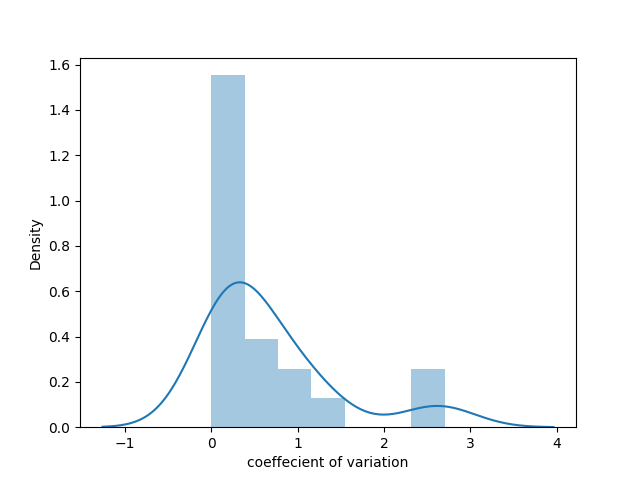
\includegraphics[scale=.5]{figure/coef_var_fig.png}
%    \caption{Graph of the density of coefficient of variation of the 20 instances}
%    \label{fig:coefVar}
%\end{figure}

%%%%%%%%%%%%%%%%%%%%%%%%%%%%%%%%%%%%%%%%%%%%%%%%%%%%%%%%%%%%%%%%%%%%%%
\section{Conclusions and perspectives}

In this paper, we have presented Lot Sizing Problems particularly the Pigment Sequencing Problem (PSP) which is a Discrete Lot Sizing Problem (DLSP). Then, We have exposed the basic concepts supporting the implementation of Genetic Algorithms. Solving a Discrete Lot Sizing Problem with Genetic Algorithms is met with some interesting challenges among which the adequate design of the chromosome or the one of the several aspects of GA such as the selection, initialization, crossover and mutation. Thanks to the instances provided by Ratheil and al [?] in their CSPLib library, we have tested our approach based on Genetic algorithms and showed that the implementation of Genetic Algorithms in solving a DLSP is a promising research area. \\
As future work, we would like to dive deeper in designing or experimenting with new approaches of crossover and mutation that respectively find better offsprings more efficiently and allow to randomly discovery promising area in the search space. It would be also interesting to test our approach on much more complex instances of several machines and a larger number of periods. 

%\begin{acknowledgment}
%ASME Technical Publications provided the format 
%\end{acknowledgment}

%%%%%%%%%%%%%%%%%%%%%%%%%%%%%%%%%%%%%%%%%%%%%%%%%%%%%%%%%%%%%%%%%%%%%%
% The bibliography is stored in an external database file
% in the BibTeX format (file_name.bib).  The bibliography is
% created by the following command and it will appear in this
% position in the document. You may, of course, create your
% own bibliography by using thebibliography environment as in
%
% \begin{thebibliography}{12}
% ...
% \bibitem{itemreference} D. E. Knudsen.
% {\em 1966 World Bnus Almanac.}
% {Permafrost Press, Novosibirsk.}
% ...
% \end{thebibliography}

% Here's where you specify the bibliography style file.
% The full file name for the bibliography style file 
% used for an ASME paper is asmems4.bst.
\bibliographystyle{asmems4}

% Here's where you specify the bibliography database file.
% The full file name of the bibliography database for this
% article is asme2e.bib. The name for your database is up
% to you.
\bibliography{asme2e}


\end{document}
